\documentclass[12pt,a4paper,titlepage]{article}
\usepackage[utf8]{inputenc}
\usepackage{fullpage}
\usepackage[english]{babel}
\usepackage{graphicx}
\usepackage{float}
\usepackage[toc,page]{appendix}
\usepackage[labelfont=bf,font=small]{caption}

% Figure numbering
\usepackage{chngcntr}
\counterwithin{figure}{section}
\counterwithin{table}{section}

% Line spacing
\usepackage{setspace}
%\onehalfspacing
\doublespacing

% Title page
\usepackage{pdfpages}

% Color
\usepackage{color}
\definecolor{bluekeywords}{rgb}{0.13,0.13,1}
\definecolor{greencomments}{rgb}{0,0.5,0}
\definecolor{redstrings}{rgb}{0.9,0,0}

% Code listings
\usepackage{listings}
\lstset{language=C++,
  showspaces=false,
  showtabs=false,
  breaklines=true,
  showstringspaces=false,
  breakatwhitespace=true,
  escapeinside={(*@}{@*)},
  commentstyle=\color{greencomments},
  keywordstyle=\color{bluekeywords},
  stringstyle=\color{redstrings},
  basicstyle=\ttfamily,
  numbers=left,
  stepnumber=1,    
  firstnumber=1,
  numberfirstline=true,
  frame=tlrb
}

% Inline code
\definecolor{codegray}{gray}{0.3}
\newcommand{\code}[1]{\indent \colorbox{codegray}{\texttt{#1}}}

\begin{document}
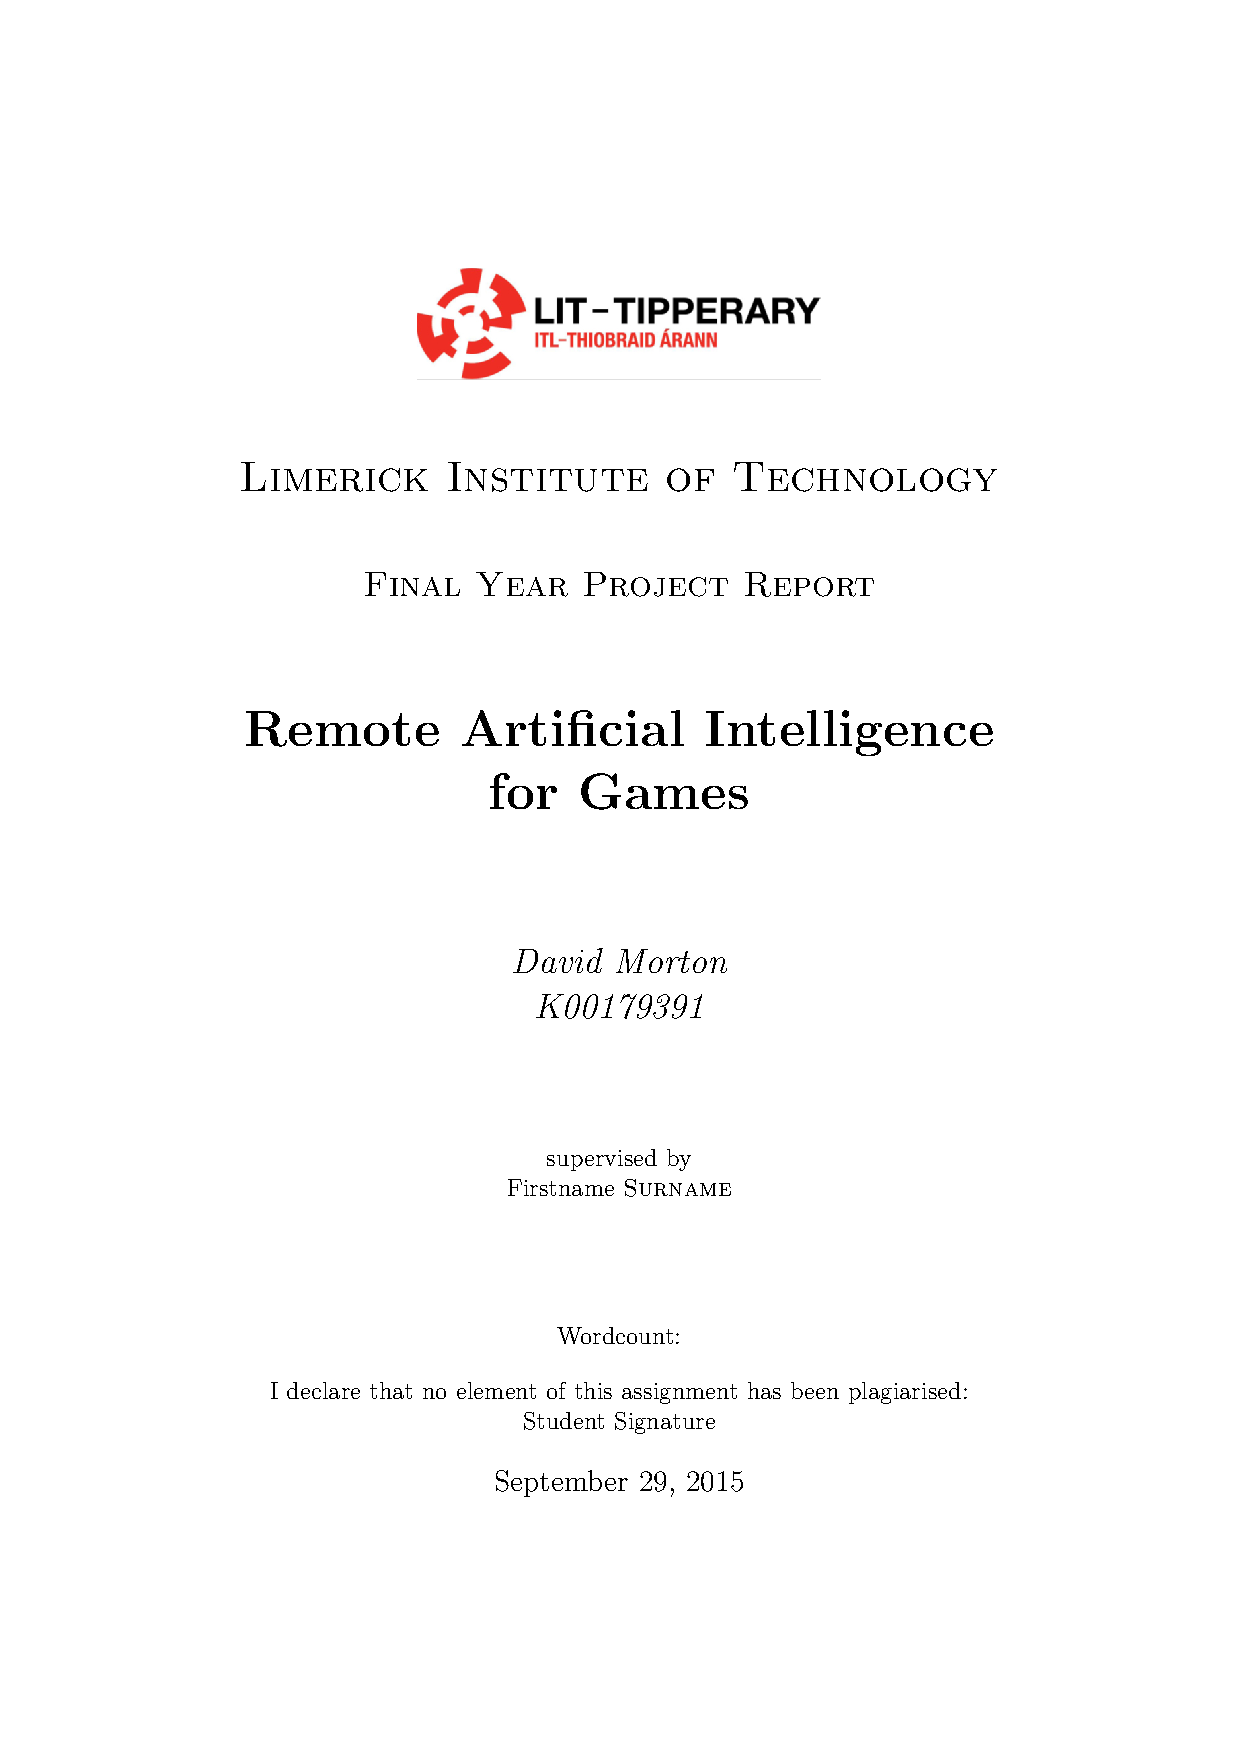
\includepdf{reportTitlePage}

% Abstract
\begin{abstract}
This is the abstract.
\end{abstract}

% Table of contents
\tableofcontents

\newpage

% List of Tables
\listoftables

\newpage

% List of figures
\listoffigures

\newpage

\section{Introduction}
\textbf{This section should contain general information on the project and the technology used.}\\

Aritificial Intelligence in games is becoming more and more popular due to new advancements in technology and increasing hardware resources on user devices. Running complex AI on users machines can sometimes be infeasible as the necessary CPU time or speed is just not available. Games are very CPU intensive applications that utilize a systems hardware for graphics rendering, audio output, networking, user inputs, and feedback. Artificial Intelligence can sometimes demand alot of processing in order to accurately generate realistic behaviours that can mimic sentient entities in a game. The type of algorithm needed for a particular behaviour in a game comes down to the knowledge and skill of the developer. This however means that highly skilled developers may attempt to implement a very complex and efficient ai algorithm when it may not be needed at all, and sometimes can produce inferior results compared to a simple animation or pre-defined behaviour. Choosing whether to use an algorithm to generate aritificial intelligence or to simply pre-define a behaviour can be very difficult and could lead to huge amounts of time and resources being wasted in a feable attempt to create SkyNet\cite{skynet}. 

Network bandwidth is also becoming cheaper to deliver to users through home broadband connections and on their mobile devices. The combination or cheap bandwidth, increased network speeds, and high performance computer hardware opens up the possibility of distributed processing for faster results from computing large data sets. Distributed processing is used to divide large datasets into smaller, more managable pieces in order to process them individually and produce results faster through the use of multiple machines connected over a network. Multiplayer games can utilize a network to run a game instance on high powered machines that will then send rendering information to the connected clients. Because aritificial intelligence algorithm processing can be intensive it makes sense to use a similar model to the client server multiplayer game to process large amounts of data on a higher end machine compared to a users mobile devices or home computers.

What this project aims to achieve is the use of the internet as a means to transmit the results of executing CPU intensive path finding algorithms used in real time strategy games on a remote server machine. Abstracting the implementations of path finding algorithms and providing developers with a simple to use Application Programming Interface that communicates with a remote server to generate results may save individually developers and studios a considerable amount of time, money, and resources. The A* pathfinding algorithm is a popular algorithm used in games to calculate paths through the games geometry. The graph consists of nodes and connections, also known as vertex and edges, with weights or values associated with each edge. Moving from one node to another node may incur a cost which is the value assigned to a connection. A* works on a non-negative weighted graph and so the game geometry must be converted into a state that the algorithm can understand. This algorithm, once it recieves the data it needs over the network, will process the data sending the result back to the client for use in the game. Many times in real time strategy games the player or enemy units will need to move from one location on the map to another along the shortest possible route while avoiding obstacles such as villages, cliffs, towers, or oceans. It would not be acceptable for the units to just cut across the map ignoring its explicit structure. 

\section{Problem Definition, Background, and Planning}

\textbf{Explain how you understand the project objective(s), what is to be solved or done, your perception of what has to be accomplished including the scope. RTS Games, controlling enemy characters. Provide a plan for the project timeline implementation including key tasks, deadlines and outputs.}\\


\subsection{Objectives}
Explain how you understand the project objective(s), what is to be solved or done, your perception of what has to be accomplished including the scope. 

\subsection{Project Planning}
Agile approach, PID, Charter, Phases.

Provide a plan for the project timeline implementation including key tasks, deadlines and outputs.

\section{Literature Review and Research}
Outline the literature reviewed and research completed to inform the completion of your project.  This should include commentary on current and emerging technologies/systems, key data, information, source, code etc. which was sourced as part of your research.  Where relevant indicate any conclusions or recommendations arising from your research

\subsection{Overview of Aritificial Intelligence in Games}

\subsubsection{Hardware Resources}

\subsubsection{Levels of Aritificial Intelligence}

\subsection{Networked Aritificial Intelligence}

\subsubsection{Distributed Client Side Processing}

\subsubsection{Central Server Architecture}

\subsection{Current Issues with Aritificial Intelligence in Games}

\subsubsection{Complex Algorithms \& Implementations}

\subsubsection{Network Latency}

\subsubsection{Human Perception}

\subsection{Conclusions of Research}

Explain the reasoning behind the decisions made for the client api, the sockets layer using TCP, the server application forking, and the AI system structure using C++ and Python.

\section{System Design and Configuration}
Describe your approach to solving the problem and, where relevant, include sub sections on

\subsection{System Architecture}

\subsection{Class Diagram}

\subsection{Sequence Diagram}

Actual code is to be provided on an accompanying and suitably labeled CD.

\section{Example of use}
How do you see the solution being used in practise? Illustrate as appropriate with User Stories / Use Cases 

\begin{figure}[H]
\begin{lstlisting}
const float TimeBetweenCameraChanges = 2.0f;
const float SmoothBlendTime = 0.75f;
TimeToNextCameraChange -= DeltaTime;
if (TimeToNextCameraChange <= 0.0f)
{
    TimeToNextCameraChange += TimeBetweenCameraChanges;

    // Find the actor that handles control for the local player.
    APlayerController* OurPlayerController = UGameplayStatics::GetPlayerController(this, 0);
    if (OurPlayerController)
    {
        if ((OurPlayerController->GetViewTarget() != CameraOne) && (CameraOne != nullptr))
        {
            // Cut instantly to camera one.
            OurPlayerController->SetViewTarget(CameraOne);
        }
        else if ((OurPlayerController->GetViewTarget() != CameraTwo) && (CameraTwo != nullptr))
        {
            // Blend smoothly to camera two.
            OurPlayerController->SetViewTargetWithBlend (CameraTwo, SmoothBlendTime);
        }
    }
}
\end{lstlisting}
	\caption{This is a code listing}
	\label{code:raig header file}
\end{figure}

And this is a reference to the code listing \ref{code:raig header file}


\begin{table}[H] %% <--- and this
\begin{center}

\begin{tabular}{ | c | c |}
\hline
A & B \\ 
\hline
C & D \\
\hline
\end{tabular}
\caption{Example table caption}
\label{table:x Example table}
\end{center}
\end{table}

This is a reference to table \ref{table:x Example table}

\begin{figure}[H]
	\centering
    	
\includegraphics[width=\textwidth]{Figures/lit_logo}
	\caption{Picture of the LIT Logo}
	\label{fig:example figure and caption}
\end{figure}

And this is a reference to the figure in Figure \ref{fig:example figure and caption}.


\section{Remote Artificial Intelligence for Games}

\subsection{Introduction}

Describe how the solution was implemented and any problems particular to this stage.

Client side API\\
Sockets layer\\
Server side application\\
AI Algorithms\\

\subsubsection{Networking Model}

Client server model\\

\subsubsection{Design Patterns}
Observer pattern\\
Stradegy pattern\\
Lazy loading\\
RAII\\

\subsection{Client API Design}

The API should be designed with developers in mind and must be intuitive to use. If a developer wants a path from A to B on their map, the API must allow the developer to quiery the service and recieve the answwer. While implementing the API the developer needs options or weigths that may determine what path is choosen for a particular situation. 

\subsubsection{Pimpl Idiom}

The Pimpl idiom is a design pattern used to hide the implemenation details of an API. A pointer to an object contained inside the .cpp implementation file removes any of the declarations and includes needed for the API header file. The implementation code is then stored in a library and the client can then link against the library when building their system. This technique can be used with proprietary code and prevents users from casually reading he header file to find out how the system is coded. 

This technique is used in the client side API for RAIG to simplify the interface for the user. APIs should be a simple as possible to support ease of use. 

\subsubsection{Game Representation}

Custom structs and contraining how the game will be presented to the AI


\subsection{BSD Sockets Layer}

\subsubsection{UDP vs TCP}

\subsubsection{Communication Protocol}

Packet header overview and details.\\

\subsection{Server System Design}

There are many ways a server systems architecture can be designed. Multiple users may need to connect and use the services provided by the server at any one time. How the server will scale to the number of users is a very important consideration when designing a remote service. This decision needs to made early in the initial envisioning phase of a project becuase it determines how the resources of the host machine will be used, how to limit or allocate more resources if needed, and also the approach taken to implement the solution.\\

\subsubsection{Benefits of Remote Processing}

Moving the graph search and processing to the server is a huge benefit to game developers. It allows the developers to forget about how the AI algorithms will run on particular systems or how much time it may take to calculate a specific query. Graph processing for state based AI is an example of a CPU intensive task, when implemented well. Removing this processing to the server frees up the resources needed for the action so they can be used elsewhere.\\


\subsubsection{Fork or Select}

Two ways to handle multiple clients connecting to a server are to \textit{fork()} a new process for each client, or using the \textit{select()} function to listen for active file descriptors. Both methods have there advantages and limitations. Forking a process to handle a client request or using select to handle requests starts with creating a listening socket on the server. 

\begin{figure}[H]

\begin{lstlisting}
sock = socket(AF_INET, SOCK_STREAM, 0); 
if (sock < 0) {
	perror("creating stream socket");
	exit(1);
}

server.sin_family = AF_INET;
server.sin_addr.s_addr = htonl(INADDR_ANY);
server.sin_port = htons(HANGMAN_TCP_PORT);

if (bind(sock, (struct sockaddr *) &server, sizeof(server)) < 0) {
	perror("binding socket");
	exit(2);
}

listen(sock, 5);
\end{lstlisting}
	\caption{This is another code listing \cite{stevensunp}}
	\label{code:raig header source}
\end{figure}

The socket is created using the \textit{socket()} function, this returns a file descriptor which is an integer value identifying the socket on the system. The \textit{SOCK\_STREAM} argument is used to create a TCP streaming socket. Next the servers address structure is filled in with details pertaining to a passive server. The \textit{htonl(INADDR\_ANY)} function on line 8, tells the server to listen for any address, IP 0.0.0.0, in order to receive incoming connection requests from any IP address. The address structure is also initialized with a port number, shown on line 9 in code listing \ref{lst:server listen}. Using the \textit{bind()} function while passing in the socket file descriptor and address structure will bind the socket to the port.\\ 

This is similar to how a client socket is created and initialized. The main differences being that the active client will use the \textit{connect()} function to connect to a passive server and will also fill in an address structure with details of the server. The server on the other hand uses the \textit{listen()} function to passively listen for incoming client connections on the port number it is bound to. \\

Once the server is running and listening for incoming clients it can handle each client request by forking a process. Forking a process starts with a parent, this parent will create child processes that will execute along side the parent and will communicate with clients using the file descriptors associated with each. When a server accepts a connection is will \textit{fork()}, this will create another process that contains a copy of the data stored in the parent process, along with the newly created file descriptor for the conenction. The parent will then close the file descriptor it has which reduces the reference count to the descriptor by 1. The child process has a copy of this information and so the child can still use the file descriptor to send and receive data. Once the child process is finished with the client communications it closes the socket, reducing the reference count to 0, and exits. The parent must then kill the process in order to aviod creating \textit{zombie} processes that have been allocated system resources but are not being used. Killing a child process involves handling signals from the kernel in the parent that identify the child process being terminated. An advantage to using \textit{fork()} over \textit{select()} is that the process can handle each client individually and does not have to worry about any more incoming connections to the server. A disadvantage to forking is that it has to uses shared memory to communicate with other processes. This can introduce concurrency issues that can be very complex, difficult to understand, and hard to debug if something goes wrong.\\

Another approach to handling client connections is to use \textit{select()}. This method will not create new processes. A single process handles all open file descriptors by looping through them and processing any that are active. The advantages of this approach over forking is that all clients are handled by a single process. This removes the need for shared memory or synchronisation primitives in order to communicate with other processes.\cite{theworldofselect} The disadvantage to using \textit{select()} over forking is that it cannot act like there is only one client at a time. With \textit{fork()} the developer can program the server as if there is only ever going to be one client which makes the code alot less complex. 



In conclusion, handling multiple clients at the server can be achieved through a variety of different ways 

\subsubsection{Round Robin DNS}

Multiple servers running instances of the AI application that can handle a number of clients each. 

\subsection{Artificial Intelligence \& Algorithms}

\subsubsection{A* Path finding}

\subsubsection{Brute force}

\subsubsection{Graph Sturctures}

Game AI is best represented as a graph like structure. Using a graph allows many different algorithms to be used to process the data efficiently.

\subsection{Analysis, Testing, and Results}

Describe the testing that was carried out and the results.

Give an account of the results of the project, what was accomplished, what wasn't and the reasons why. If the project is incomplete or has potential for improvement state what further features could be included and how existing ones might be improved.

Google C++ testing framework

\subsection{Summary}


\section{User manual (where appropriate)}
Write a concise but complete user manual or guide. This can be light on text so long as a novice user has enough information to use the application unaided.

LaTeX\\
doxygen\\
Make\\
MetaUML\\
UMLet\\

\section{Critical analysis, Conclusions, and Future Work}

Evaluate the success of what was achieved against the original objectives. 

What difficulties were encountered and what lessons learned from the project? 

How well did the project follow the planned timeline and how useful was the timeline?  

What are your key conclusions from the work.?

This is a reference to the graph appendix \ref{appendix:graph}

This is a reference to the Network Programming Book \cite[p.~215]{stevensunp}

% References
\newpage

\begin{thebibliography}{99}
\addcontentsline{toc}{section}{References}

\bibitem{skynet}
Skynet (Terminator) - Wikipedia, the free encyclopedia. 2015. [ONLINE] Available at: \textit{https://en.wikipedia.org/wiki/Skynet\_(Terminator).} [Accessed 09 October 2015].

\bibitem{stevensunp}
W. Richard Stevens, 2003. \textit{Unix Network Programming, Volume 1: The Sockets Networking API (3rd Edition)}. 3 Edition. Addison-Wesley Professional.

\bibitem{theworldofselect}
The World of select(). 2015. The World of select(). [ONLINE] \\
Available at: \texttt{http://www.lowtek.com/sockets/select.html.} [Accessed 01 October 2015].

\end{thebibliography}



% Appendices
\newpage
\begin{appendices}

\section{Graph Appendix}
\label{appendix:graph}
This is the graph appendix...

\section{Another Appendix}

\end{appendices}

\end{document}